\RequirePackage{xcolor}

\documentclass[usletter,11pt,final]{article}

\usepackage[utf8]{inputenc}
\usepackage[T1]{fontenc}
\usepackage{hyperref}
\usepackage[caption=false]{subfig}
\usepackage{textcomp}
\usepackage{tikz}
\usepackage{cite}
\usepackage{amssymb}
\usepackage{amsmath}

\title{Notes}
\author{Vincent Billaut}
\date{\today}

\begin{document}

\begin{titlepage}
\maketitle
\tableofcontents
\end{titlepage}

\section{Revealing common elements in independent string sets}
\subsection{Definition of the problem}

We have a set of nodes $A_i$ that each have $p_i$ strings $S_{i,k}$, and every node is connected to the central hub $C$, which is the only way for them to communicate with each other.

\begin{figure}[h]
\begin{center}
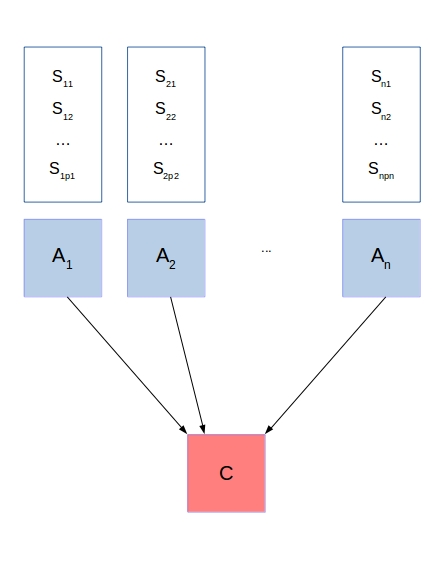
\includegraphics[width=200px]{img/sketch1.jpg}
\caption{Visualization of the problem}
\end{center}
\end{figure}

The problem is that a node $A_i$ wants to know whether they have \textbf{a string $S$ in common} with another node $A_j$ ($i \ne j$), without the other ones having that information, and without knowing which $j$.

To achieve this, $A_i$ can send a query $Q$ to $C$ and gather the responses from the $A_j$, $j \ne i$. Only $C$ and $A_i$ see the responses. $A_i$ should then be able, based on $Q$ and on those responses, to determine whether one has a string in common with it. The other $A_j$ cannot know about the result, and cannot be shown sensitive information (such as the $S_{i,k}$).

Let's assume in what follows that $A_1$ is the one issuing the query.

\paragraph{Application to genomics} The problem is set in an abstract way, but intended to solve a very practical issue in the field of genomics. The nodes represent centers that have large amounts of genome sequences taken from patients (we won't focus on the format of those sequences for now). The problem aims at enabling cooperation between the centers without any confidential information disclosure. If a physician wants to use all the data available to compute statistics on a given gene, it is critical information to know whether a given patient appears several times in the dataset. This is impossible today, because the centers don't share that information. We're focusing here on a non-intrusive way to determine that two centers possess the information from the same individual.

\subsection{Hashing function}
\subsubsection{Description}
A simple way would be for $A_1$ to use a hashing function.
\begin{itemize}
\item $A_1$ chooses a hashing function $h$; this is a one-way function from the space of strings ($\mathbb{S}$) to a finite set of integers (from 1 to $N$); the ideal hashing function spreads the inputs \textbf{uniformily} across the possible values;
\item $A_1$ broadcasts $h$ to the other nodes, through $C$;
\item $\forall i \ne 1, A_1$ gathers $\mathbb{H}_i =  \{h(S_{i,k}), 1 \le k \le p_i\}$ \textbf{without knowing from which $A_j$ those come from};
\item $A_1$ checks whether $\exists j, \mathbb{H}_1 \cap \mathbb{H}_j = \varnothing$; if so, it concludes that it has a string in common with an $A_j$ and retrieves it; if not, it concludes that they have no string in common with any other $A_j$.
\end{itemize}

In what follows, we will consider the case where we only have $A_1$ and $A_2$, so $A_1$ just wants to know whether it has a common string with $A_2$.

With an ideal hashing function that would guarantee $x \ne y \Rightarrow h(x) \ne h(y)$, the method described above is valid.

The problem arises when we take into account the probability of collision of $h$ (ie the probability of having the same hash for two different strings).  In particular, if $$\exists k,k' \quad \textrm{s.t.} \quad S_{1,k} \ne S_{2,k'} \quad \textrm{and} \quad h(S_{1,k}) = h(S_{2,k'})$$ then $A_1$'s conclusion is misguided.

However, in our setup, it is impossible to "miss" a string in common. If $\mathbb{H}_1 \cap \mathbb{H}_2 = \varnothing$ then we know there is none. The only issue consists in deciding, when $\mathbb{H}_1 \cap \mathbb{H}_2 \neq \varnothing$, whether the equality of hashed values is due to the strings being the same or to a collision in the hashing function.

\subsubsection{Statistical approach}

\paragraph{Testing setup}
Our goal here is to determine whether there is a common string in $A_1$ and $A_2$. In order to do that, we will design a statistic, determine a way to answer the question based on that statistic (this is the test function) and derive confidence metrics around the decisions we make.

Basically, we set $H_0$: \textit{there is no common string between $A_1$ and $A_2$} against $H_1$: \textit{there exists at least one string in common between $A_1$ and $A_2$}. We will see what a relevant statistic for this problem is, and what its behaviour under $H_0$ is.

\paragraph{Our model}
The natural way to model the hashing function is to represent the output of $h$ as a random variable $U$. Our hypothesis is that $h$ is a \textit{good} hashing function, which translates into the assumption that \textbf{$U$ is uniformely distributed across $[1 .. N]$}.

Let $U_1, ..., U_{p_1}$ and $U_1', ..., U_{p_2}'$ be the hashed strings of pools $A_1$ and $A_2$. The $U$ and $U'$ are iid and $U_i \sim U$.
The idea of avoiding collisions leads us to consider the following statistic: $$ S = \sum_{i=1}^{p_1} \sum_{j=1}^{p_2} 1_{U_i = U_j'} $$ which counts the number of collisions.

We could be tempted to assess that $S \sim B(p_1 p_2, \frac{1}{N})$, where $B(n,p)$ denotes a Binomial distribution of parameters $n$ and $p$, but we can actually easily see that the $1_{U_i = U_j'}$ are \textit{not} independent. Indeed, we have that $$ \forall i,j \quad E(1_{U_i = U_j'})=\frac{1}{N} $$ but notice that $$ \forall i,j \quad E(1_{(U_i = U_j')} \quad | 1_{(U_i = U_i')}=1_{(U_j = U_j')}=1_{(U_j = U_i')}=1) = 1$$

The easy way to think about this is to consider the issue purely as a counting problem.

\paragraph{Counting approach}
If we consider that our hashing function evenly distributes values across integers between 1 and $N$, then the probability of a collision within a set of $n$ hashed values is known\footnote{this is a generalized version of the birthday problem (\url{https://en.wikipedia.org/wiki/Birthday_problem})}: 

\begin{equation}
\begin{aligned}
\textrm{P}(collision) & = 1 - \prod_{k=1}^{n-1} (1 - \frac{k}{N}) \\
					  & \approx 1 - e^{- \frac{n^2}{2N}}
\end{aligned}
\end{equation}

We can generalize this, considering two different sets (here, the strings of $A_1$ and $A_2$) and evaluating the probability of having a collision across them, and the result is particularly complicated (see \cite{WENDL2003249}). For now, let's just look at the probability of there being a collision in the union of $A_1$'s and $A_2$'s hash sets. Of course, this is the probability of a collision with the prior that there is no common string between $A_1$ and $A_2$ (that is, the probability of wrongly concluding that there is a common string). $$\textrm{P}(\exists H,H' \in \mathbb{H}_1 \cup \mathbb{H}_2 \quad H=H'  | \forall i,j \quad S_{1,i} \ne S_{2,j}) \approx 1 - e^{- \frac{(p_1+p_2)^2}{2N}}$$

In fact we have that if $k-1$ values are already drawn, the probability that the $k^{th}$ value will repeat one of the previous ones is $q(k,N) = 1 - (\frac{N-1}{N})^{k-1}$. We can consider here that $p_1$ values are drawn, and that we repeat the experiment of pulling a $(p_1+1)^{th}$ independently $p_2$ times. That way, we can compute the expected number of collisions of our experiment:

\begin{equation}
\begin{aligned}
\textrm{E}(\#collisions)  & = p_2 \left(1 - \left(\frac{N-1}{N}\right)^{p_1}\right)\\
					   & \approx \frac{p_1 p_2}{N}
\end{aligned}
\end{equation}

Instinctively, we see that if $p_1 p_2 \ll N$, observing one collision between the hashed values of $A_2$ and those of $A_1$ would be strong evidence for the conclusion that there is a common string.

\paragraph{Back to statistics}
Those observations tend to suggest to use another statistic for our test. We define $S$ as $$S = \sum_{i=1}^{p_2} 1_{U_i' \in \mathbb{U}_1}$$ where $\mathbb{U}_1$ denotes the set $\{U_1, ..., U_{p_1}\}$.

Under $H_0$, those observations are independant and each correspond to a Bernoulli trial of probability $p = q(p_1+1,N)$.
The statistic $S$ therefore follows a Bernoulli distribution of parameters $p_2$ and $q(p_1+1,N)$, namely $$ S \sim B(p_2, \left(1 - \left(\frac{N-1}{N}\right)^{p_1}\right))$$

\paragraph{Note} We find $E(S) = p_2 \left(1 - \left(\frac{N-1}{N}\right)^{p_1}\right)$ as expected.

\vspace{5mm}
Basically, we now have the information that under $H_0$: $$S \sim B(p, q_0)$$ with $p = p_2$ and $q_0=q(p_1+1,N)$, and we want to test that (under $H_1$ the distribution looks different, because the string in common will arise way sooner than any collision would).

Therefore, we need to perform a goodness-of-fit test (for instance a Pearson's $\chi^2$ test\footnote{See \url{https://en.wikipedia.org/wiki/Pearson's_chi-squared_test}}). Given the distribution at hand, and especially the fact that $q_0 \lll 1$, the test will consist in assessing, in case a collision appears, whether it is likely or not and to what extent. If $A_1$ and $A_2$ have a string in common, intuitively, we will spot it way sooner than any collision would have occurred.
If we end up with $S=0$, there is no string in common between $A_1$ and $A_2$ anyway.

\subsubsection{Extension to multiple hashing functions}
A simple extension of this solution, that would most likely solve the collision issue, is to consider multiple hashing functions. Instead of sending $h$ to the other nodes, $A_1$ sends $(h_1, h_2, ..., h_H)$ a set of $H$ hashing functions and then gathers, for each other node, $$ \widetilde{\mathbb{H}}_i = \{[h_1(S_{i,k}), ..., h_H(S_{i,k})], \quad 1 \le k \le p_i\}$$

That way, the test now consists in comparing not only one hashed value, but $H$ hashed values for each string. A collision is now characterized by the simultaneous occurrence of $H$ individual collisions (that is, having each of the $H$ hashing functions return the same output for the same two inputs). Once again, the same string in both $A_1$ and $A_2$ will produce the same output, ie the same $H$ values.

We don't change the method \textit{per se}, but we make sure to (most likely) avoid collisions. It is possible to compute the new probabilities of collision, but the argument is that it's pretty obvious that such a method is very robust.

\section{Tolerance to errors}

The previous problem is very ideally set. We assumed perfect communication between the hub and the nodes, we were looking for perfect matches between strings, etc.

If we want to tackle real problems, we need to take into account real-world specificities. For instance, we want to build a tolerance for errors in the strings we compare.

\paragraph{Application to genomics} Taking errors into account is crucial in genomics. Indeed, \cite{wall2014estimating} shows that with the democratisation of whole-genome sequencing studies come non-negligeable error rates, which makes our previous problem setting a bit optimistic, since we're looking for exact matches between sequences. If two sequences are identical at every position but one (say, if there was a single error in getting one of them), the hash function yields completely different outputs, and we therefore cannot conclude anything about the two strings.

\subsection{Complexification of the previous problem}

We build upon the previous problem: we still have a node $A_i$ that wants to determine whether it has a common string with another node $A_j$.

The difference is that now we don't suppose that the strings $S_{i,k}$ need to be exactly equal. Instead, we will take into account errors made in storing the sequences, in order to embed some tolerance into our model. In other words, we want a model that detects \textit{close similarity} between the $S_{i,k}$, in a sense that we have yet to define. To achieve that, we need to look more precisely into what the $S_{i,k}$ look like, and will right away consider the situation we're interested in.

Let $s \in \mathbb{S}$. We write $s$ as a sequence: $$s = s_1s_2...s_{n_s}$$ with $\forall k, s_k \in \{0,1,2\}$.

\paragraph{Note} The $s_k$ represent the expression of one gene for the given patient. It comes from the two representations of the gene in the patient's genome (from the two parents). It can only be 0 (reference value for both), 1 (one reference value and one alternate value) or 2 (alternate value for both).

\vspace{5mm}
The equality between two elements of $\mathbb{S}$ as considered before would be defined as $$ \forall s,t \in \mathbb{S} \quad s = t \Leftrightarrow \forall i, s_i=t_i$$

We now introduce the possibility of there being errors within the sequence. Let $\tilde{s}$ be the sequence $s$, potentially with errors (we consider $s$ to be the ground truth). We make the assumption that for each gene on any of the two parents' sequences there is a probability $\epsilon$ that the expression we have is wrong. That is, $\forall i,~ \textrm{P}(\tilde{p}_i \neq p_i) = \epsilon$ (if $p$ is a parent's sequence). These events are independent. Since $s$ is the sum of the parents' sequences, so the errors add up. We will not take into account second order errors (we have $\textrm{P}(|\tilde{s}_i - s_i| = 2) \sim \epsilon^2$) and focus on first order: $$\forall i ~ \rm P (|\tilde{s}_i - s_i| = 1) = 2\epsilon$$

For our given sequence $s$, we have an expected number of errors of $2n_s\epsilon$ (the number of errors follows a Bernoulli law).

\subsection{Locality Sensitive Hashing}

Building on our previous solutions, a way to adapt to our new constraint would be to use hash functions that have similarity-conserving properties. 

\subsubsection{General idea}

\textit{Locality Sensitive Hashing} (LSH), introduced in \cite{indyk1998approximate}, and also discussed in \cite{cohen2001finding}, aims at solving the Nearest Neighbors (NN) problem in very high dimensional data spaces (very much like the one we're focused on). The idea is to build a hash function that will map similar vectors to the same value, thus building similarity clusters. Apart from NN, this property can be used for error-tolerant hashing. Indeed, we expect that the most similar vector pairs are actually pairs of two flawed versions of the same vector. We expect that different vectors will never get as close to each other as a vector and itself with errors.

Given a similarity function $S$, for instance based on the Hamming distance $d_H$\footnote{In this case, the similarity is defined as $S(s,q)= \frac{|s|+|q|-d_H(s,q)}{|s|+|q|+d_H(s,q)} $} (discussed in \cite{cohen2001finding}, 4.3), the property of the LSH function $h$ is $$ \rm P(h(s)=h(q))=S(s,q) $$

Building an LSH function requires to set some sort of threshold. Intuitively, if we simplify the view to a deterministic  setting, the threshold $c$ can be interpreted as follows: $S(s,q) > c \Leftrightarrow h(s) = h(q)$.

\paragraph{Note} We see right here that setting a threshold can be useful to extend our problem. If we suddenly decide to not only spot duplicates between silos, but also get a sense of whether the data about a patient's close family members is available in other silos, we can then modify the threshold accordingly. Moreover, using many LSH functions, each with a different threshold, would constitute a way to assess the proximity between two strings, without having access to them.


\vspace{5mm}
What's interesting about LSH functions is that they come in families. All the functions in a family share a property, but each has its own parameters and thresholds. Rigorously, the threshold of a given LSH function can be defined, for any $\epsilon,\delta,R>0$, as: 

\begin{equation}
\begin{aligned}
d(s,q) \le (1 - \delta)R \quad & \Longrightarrow \quad \rm P(h(s)=h(q)) \ge 1-\epsilon\\
d(s,q) \ge (1 + \delta)R \quad & \Longrightarrow \quad \rm P(h(s)=h(q)) \le \epsilon
\end{aligned}
\end{equation}

(where $d$ is the distance function ; we could have also used a similarity function)



\paragraph{Note} \cite{jbuhler} introduces an interesting \textit{locality-sensitive} method to perform genetic sequence comparison and retrieve similar sequences. The issue when we want to use it in our case is that it requires full access to all the strings at hand. In the context of inter-silo information sharing, matters of privacy, confidentiality and accessibility come into play, rendering the \textsc{LSH-ALL-PAIRS} algorithm moot.

\subsubsection{Building our own LSH function}

\paragraph{Observation}

In order to build a relevant, robust LSH function for our particular case, we need to look at the behavior of the data at hand and particularly at the similarity distribution amongst the pairs of genomic sequences that we can find in the silos.

We choose to focus, for this exploration, on the chromosome \#22 (because of its rather small size). We pull the data from \url{ftp://ftp.1000genomes.ebi.ac.uk/vol1/ftp/phase1/analysis_results/integrated_call_sets/} and retrieve two sets of genomic data of size $N$ (number of patients). Each genome sequence here has length over 450,000.

In the following, we will be using the \textbf{Hamming distance}, which represents the number of substitutions needed to go from one sequence to the other. In a genetics context, this is very relevant. More precisely, we will consider the \textbf{Hamming similarity}, which is derived from the Hamming distance (we gave its definition above). What we're interested in is understanding how close to each other different sequences are. For a given patient, what is the distribution of similarity between that patient and all the others? This distribution (shown in Figure \ref{indivhist}) has a normal shape, fading away long before reaching 1. This suggests that we can introduce a level of confidence by accepting as the same sequence two sequences with very high similarity (for instance, around 96\% or 98\%).

\begin{figure}
\begin{center}
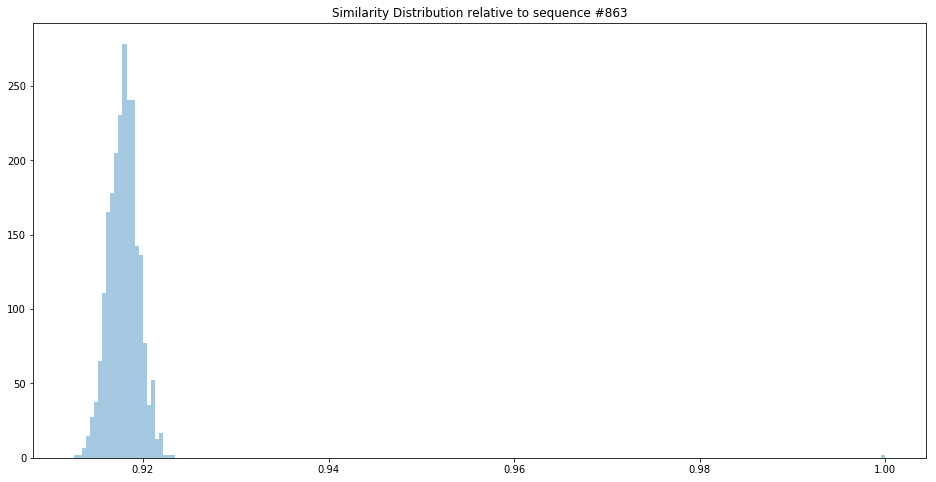
\includegraphics[height=200px]{indivhist.png}
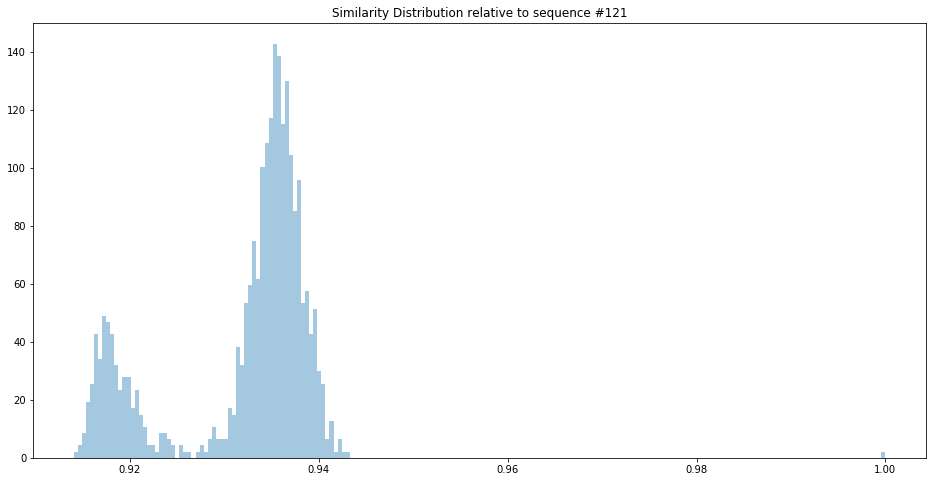
\includegraphics[height=200px]{indivhist121.png}
\caption{Similarity distributions relative to one sequence ; the distributions exhibit normal behaviour, and leave a lot of space for small mistakes (between 96\% and 100\% roughly)}
\label{indivhist}
\end{center}
\end{figure}

But this is only on haploid data. If we aggregate the two haploid sequences for each patient, and look for the same plot for the diploid sequences, the distribution will appear even further away from 1, as shown in Figure \ref{diplhist}.


\begin{figure}
\begin{center}
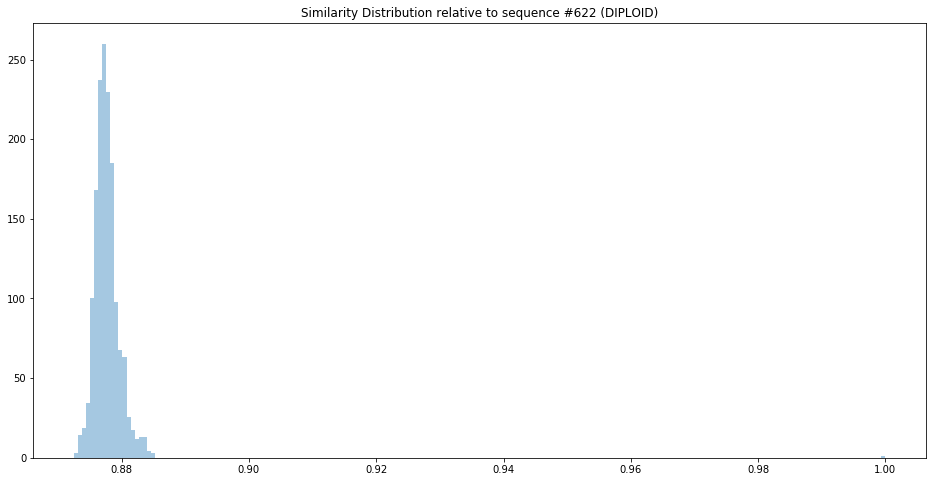
\includegraphics[height=200px]{indivhistdipl.png}
\caption{Similarity distribution relative to one diploid sequence}
\label{diplhist}
\end{center}
\end{figure}

\paragraph{Errors}

Now that we have a feeling about what a correct comparison distribution looks like, let's imagine what errors could bring into the picture. Say we have a chance $\epsilon$ of having a mistake at a given position of the sequence. If we consider two sequences $s$ and $s'$, that only differ by errors, we have:
$$ \textrm{E}(d_H(s,s')) = \epsilon \cdot l$$
with $|s|=|s'|=l$.

Therefore $$ \textrm{E}(S_H(S,s')) = {2-\epsilon \over 2+\epsilon} = 1 - \frac{\epsilon}{1+\epsilon/2}$$ which translates, with approximation that $\epsilon \ll 1$, to $$ \textrm{E}(S_H(s,s')) \simeq 1 - \epsilon$$

The law of the distance to erroneous duplicates is a binomial law of parameters $l$ and $\epsilon$, and with $\epsilon \ll 1$, the law of the similarity is similarly shaped (but reversed).

\begin{figure}
\begin{center}
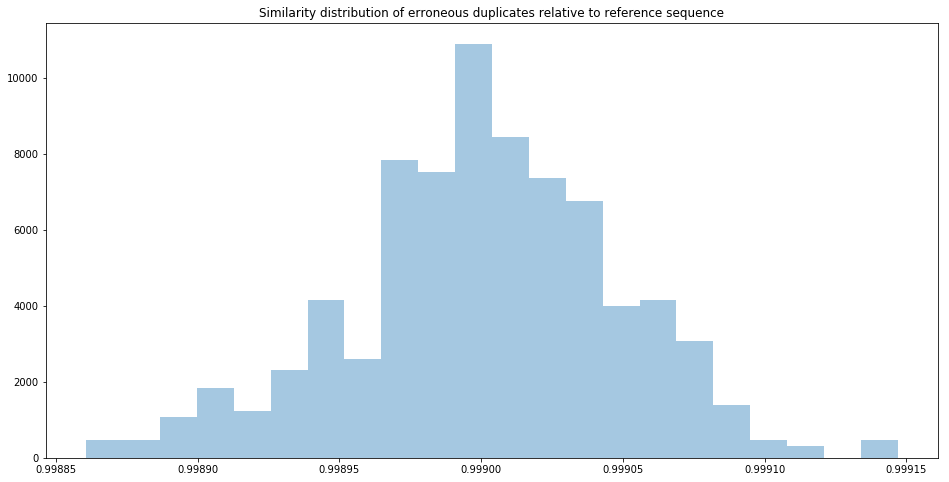
\includegraphics[height=200px]{errors.png}
\caption{Similarity distribution of simulated erroneous duplicates (haploid sequences) with $\epsilon = 0.001$}
\label{errors}
\end{center}
\end{figure}


A typical error rate being around 0.1\%, this result shows that two sequences from the same patient should have similarities around 99.9\%, which is very satisfying considering the distributions at hand. To demonstrate that, we can simulate erroneous duplicates of a random sequence and plot the resulting similarity distribution (shown in Figure \ref{errors}).

\begin{figure}
\begin{center}
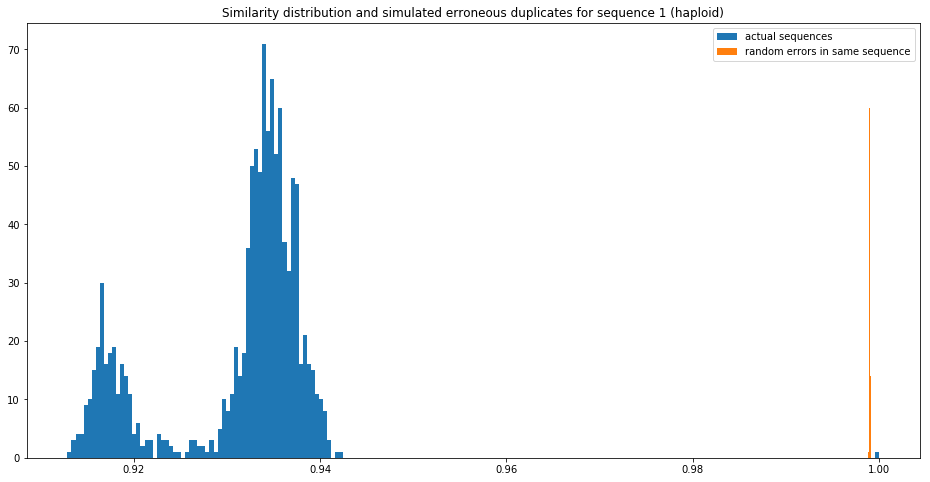
\includegraphics[height=200px]{comphist.png}
\caption{Similarity distribution of simulated erroneous duplicates, plotted with the actual similarity distribution (haploid sequences) with $\epsilon = 0.001$}
\label{comphist}
\end{center}
\end{figure}

The difference between the similarity of legit different sequences and duplicates with mistakes is pretty obvious to spot, and is visualized in Figure \ref{comphist}.

\paragraph{Building our LSH function}

\newpage
\addcontentsline{toc}{section}{References}
\bibliography{references}
\bibliographystyle{plain}

\end{document}